% https://www.stringology.org/DataCompression/lz78/index_en.html#:~:text=Description,index%20instead%20of%20the%20phrase.
LZ78-based schemes work by entering phrases into a dictionary and then, when a repeat occurrence of that particular phrase is found, outputting the dictionary index instead of the phrase.

\begin{figure}[ht]
    \centering
    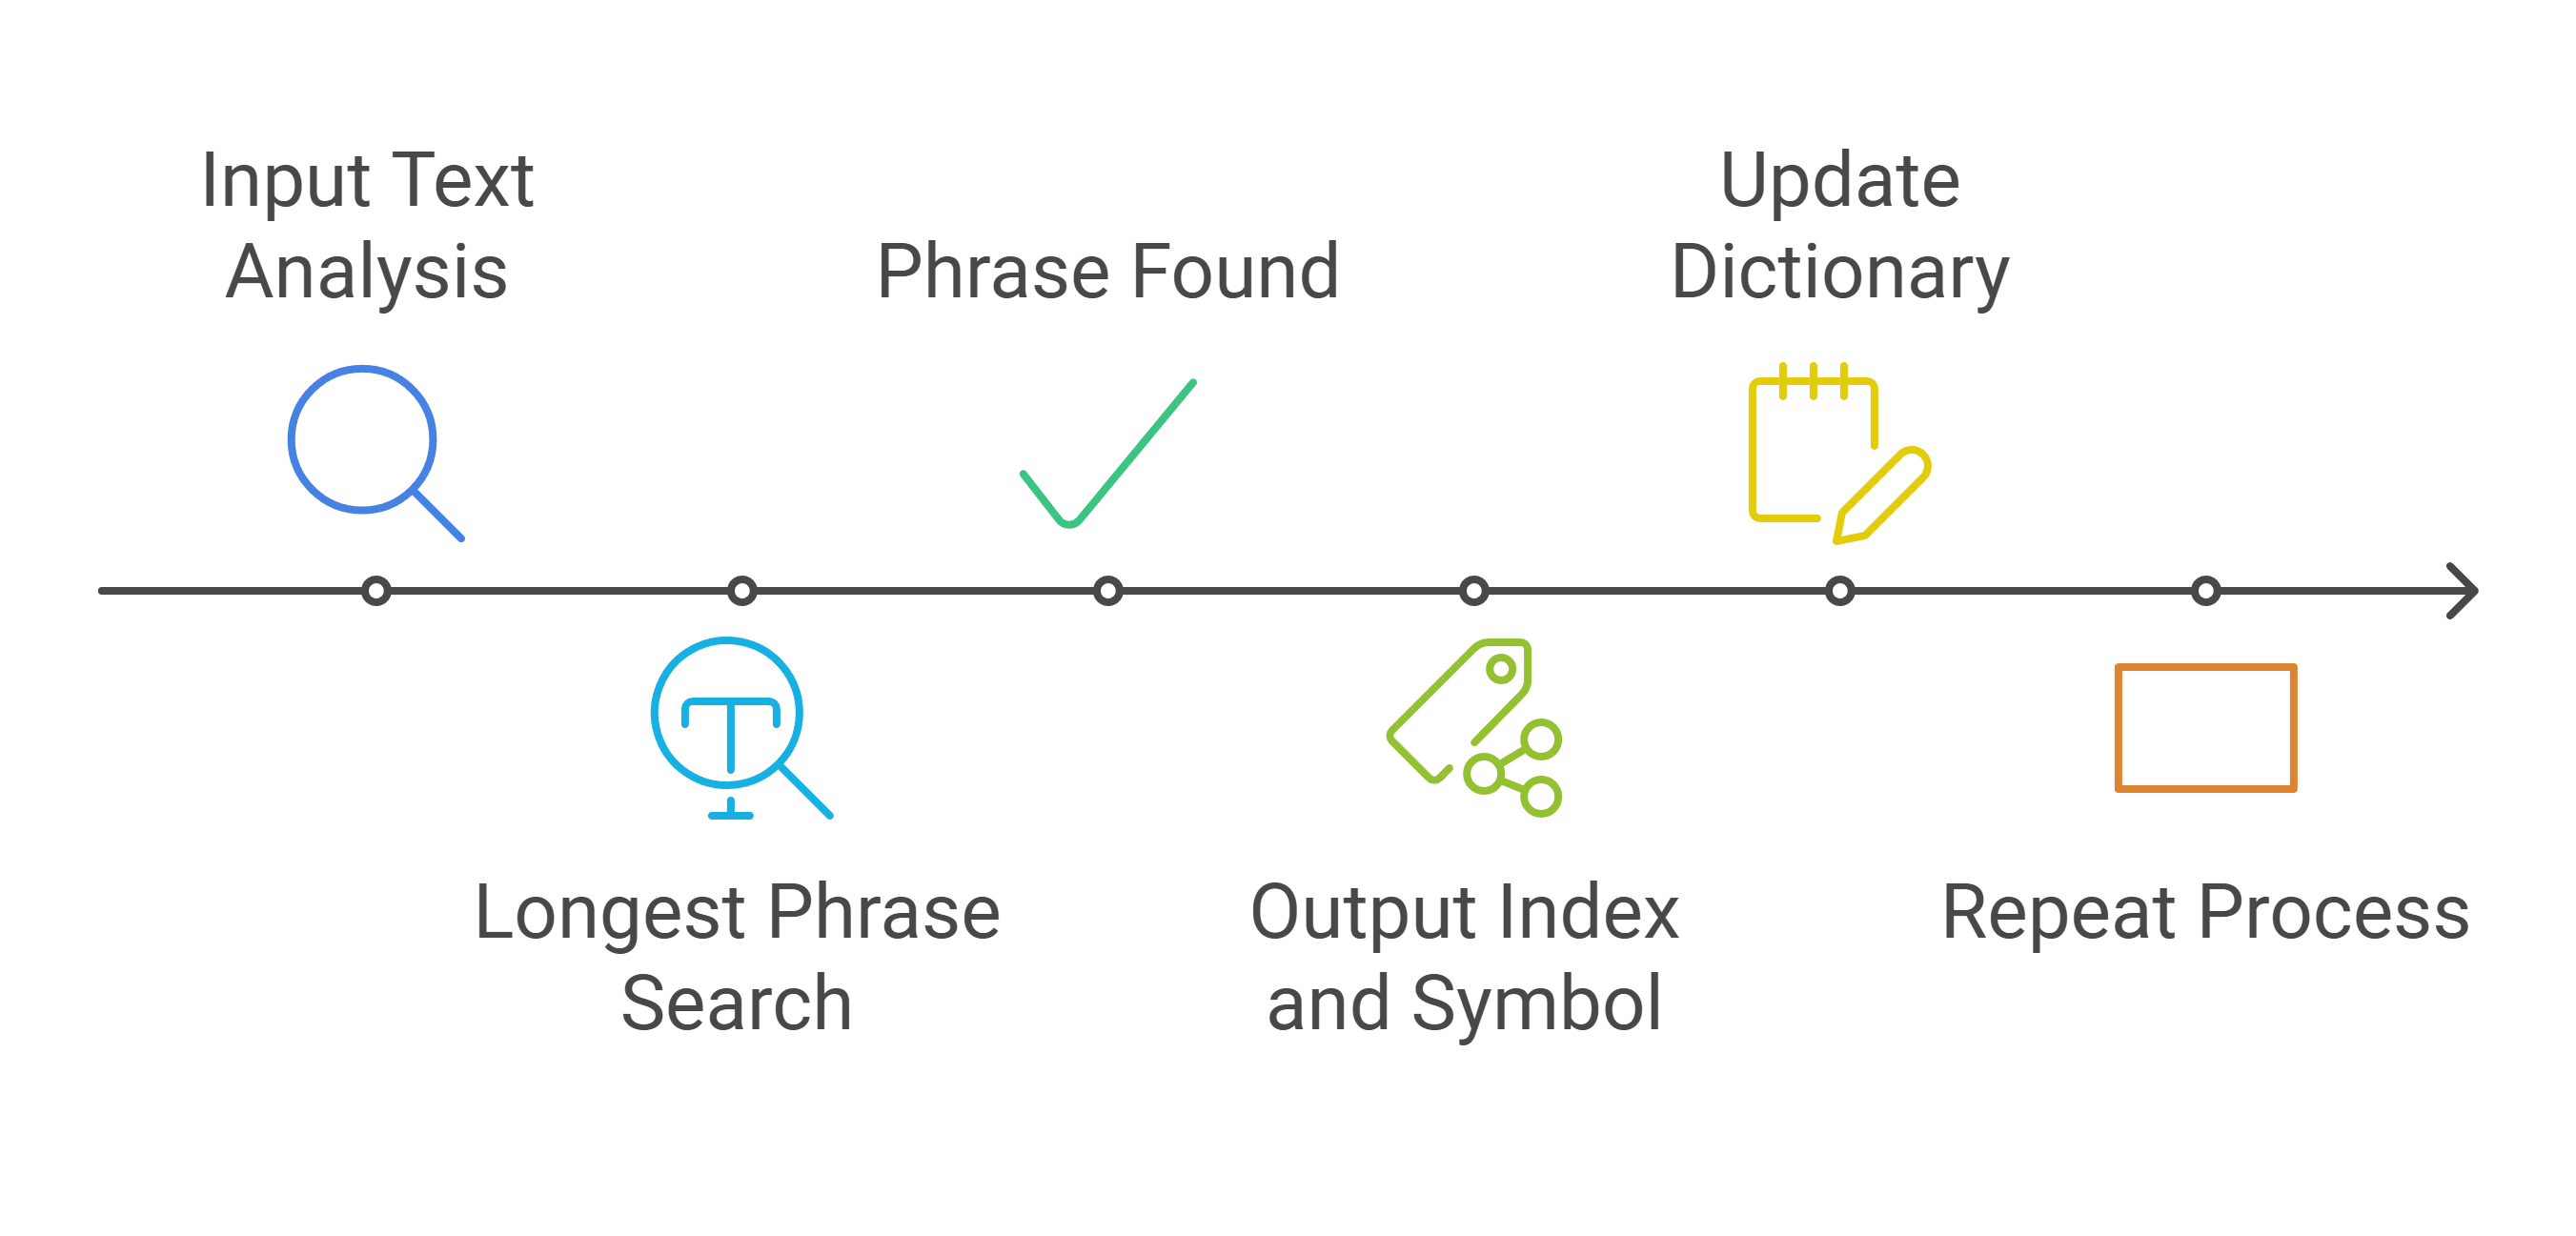
\includegraphics[width=1\linewidth]{Figures/LZ78.png}
    \caption{LZ78 Compression Process}
    \label{fig:lz78}
\end{figure}

At each step, LZ78\cite{doc5} outputs a pair (\textit{i, a}), where \textit{i} is the index of the phrase in the dictionary and \textit{a} is the next symbol following the phrase. The dictionary is represented like the trie with numbered nodes. If we go from the root to a certain node, we will get a phrase from the input text.

\vspace{10pt}
In each step, we look for the longest phrase in the dictionary, that would correspond to the unprocessed part of the input text. The index of this phrase together with the symbol, which follows the found part in the input text, is then sent to the output. The old phrase extended by the new symbol is then put into the dictionary. This new phrase is numbered by the smallest possible number.